\documentclass[journal,12pt,twocolumn]{IEEEtran}

\usepackage{setspace}
\usepackage{gensymb}
\singlespacing
\usepackage[cmex10]{amsmath}

\usepackage{amsthm}

\usepackage{mathrsfs}
\usepackage{txfonts}
\usepackage{amsmath}
\usepackage{stfloats}
\usepackage{float}
\usepackage{bm}
\usepackage{tikz}
\usepackage{pgfplots}
\usepackage{cite}
\usepackage{cases}
\usepackage{subfig}

\usepackage{longtable}
\usepackage{multirow}

\usepackage{enumitem}
\usepackage{mathtools}
\usepackage{steinmetz}
\usepackage{tikz}
\usepackage{circuitikz}
\usepackage{verbatim}
\usepackage{tfrupee}
\usepackage[breaklinks=true]{hyperref}
\usepackage{graphicx}
\usepackage{tkz-euclide}

\usetikzlibrary{calc,math}
\usepackage{listings}
    \usepackage{color}                                            %%
    \usepackage{array}                                            %%
    \usepackage{longtable}                                        %%
    \usepackage{calc}                                             %%
    \usepackage{multirow}                                         %%
    \usepackage{hhline}                                           %%
    \usepackage{ifthen}                                           %%
    \usepackage{lscape}
\usepackage{multicol}
\usepackage{chngcntr}
\usepackage{hyperref}
\hypersetup{
    colorlinks=true,
    linkcolor=blue,
    filecolor=blue,
    urlcolor=blue,
}
\DeclareMathOperator*{\Res}{Res}

\renewcommand\thesection{\arabic{section}}
\renewcommand\thesubsection{\thesection.\arabic{subsection}}
\renewcommand\thesubsubsection{\thesubsection.\arabic{subsubsection}}

\renewcommand\thesectiondis{\arabic{section}}
\renewcommand\thesubsectiondis{\thesectiondis.\arabic{subsection}}
\renewcommand\thesubsubsectiondis{\thesubsectiondis.\arabic{subsubsection}}


\hyphenation{op-tical net-works semi-conduc-tor}
\def\inputGnumericTable{}                                 %%

\lstset{
%language=C,
frame=single,
breaklines=true,
columns=fullflexible
}

\makeatletter
\setlength{\@fptop}{0pt}
\makeatother

\begin{document}


\newtheorem{theorem}{Theorem}[section]
\newtheorem{problem}{Problem}
\newtheorem{proposition}{Proposition}[section]
\newtheorem{lemma}{Lemma}[section]
\newtheorem{corollary}[theorem]{Corollary}
\newtheorem{example}{Example}[section]
\newtheorem{definition}[problem]{Definition}

\newcommand{\BEQA}{\begin{eqnarray}}
\newcommand{\EEQA}{\end{eqnarray}}
\newcommand{\define}{\stackrel{\triangle}{=}}
\bibliographystyle{IEEEtran}
\raggedbottom
\setlength{\parindent}{0pt}
\providecommand{\mbf}{\mathbf}
\providecommand{\pr}[1]{\ensuremath{\Pr\left(#1\right)}}
\providecommand{\qfunc}[1]{\ensuremath{Q\left(#1\right)}}
\providecommand{\sbrak}[1]{\ensuremath{{}\left[#1\right]}}
\providecommand{\lsbrak}[1]{\ensuremath{{}\left[#1\right.}}
\providecommand{\rsbrak}[1]{\ensuremath{{}\left.#1\right]}}
\providecommand{\brak}[1]{\ensuremath{\left(#1\right)}}
\providecommand{\lbrak}[1]{\ensuremath{\left(#1\right.}}
\providecommand{\rbrak}[1]{\ensuremath{\left.#1\right)}}
\providecommand{\cbrak}[1]{\ensuremath{\left\{#1\right\}}}
\providecommand{\lcbrak}[1]{\ensuremath{\left\{#1\right.}}
\providecommand{\rcbrak}[1]{\ensuremath{\left.#1\right\}}}
\theoremstyle{remark}
\newtheorem{rem}{Remark}
\newcommand{\sgn}{\mathop{\mathrm{sgn}}}
\providecommand{\abs}[1]{$\left\vert#1\right\vert$}
\providecommand{\res}[1]{\Res\displaylimits_{#1}}
\providecommand{\norm}[1]{$\left\lVert#1\right\rVert$}
%\providecommand{\norm}[1]{\lVert#1\rVert}
\providecommand{\mtx}[1]{\mathbf{#1}}
\providecommand{\mean}[1]{$E\left[ #1 \right]$}
\providecommand{\fourier}{\overset{\mathcal{F}}{ \rightleftharpoons}}
%\providecommand{\hilbert}{\overset{\mathcal{H}}{ \rightleftharpoons}}
\providecommand{\system}{\overset{\mathcal{H}}{ \longleftrightarrow}}
	%\newcommand{\solution}[2]{\textbf{Solution:}{#1}}
\newcommand{\solution}{\noindent \textbf{Solution: }}
\newcommand{\cosec}{\,\text{cosec}\,}
\providecommand{\dec}[2]{\ensuremath{\overset{#1}{\underset{#2}{\gtrless}}}}
\newcommand{\myvec}[1]{\ensuremath{\begin{pmatrix}#1\end{pmatrix}}}
\newcommand{\mydet}[1]{\ensuremath{\begin{vmatrix}#1\end{vmatrix}}}
\newcommand*{\permcomb}[4][0mu]{{{}^{#3}\mkern#1#2_{#4}}}
\newcommand*{\perm}[1][-3mu]{\permcomb[#1]{P}}
\newcommand*{\comb}[1][-1mu]{\permcomb[#1]{C}}
\numberwithin{equation}{subsection}
\makeatletter
\@addtoreset{figure}{problem}
\makeatother
\let\StandardTheFigure\thefigure
\let\vec\mathbf
\renewcommand{\thefigure}{\theproblem}
\def\putbox#1#2#3{\makebox[0in][l]{\makebox[#1][l]{}\raisebox{\baselineskip}[0in][0in]{\raisebox{#2}[0in][0in]{#3}}}}
     \def\rightbox#1{\makebox[0in][r]{#1}}
     \def\centbox#1{\makebox[0in]{#1}}
     \def\topbox#1{\raisebox{-\baselineskip}[0in][0in]{#1}}
     \def\midbox#1{\raisebox{-0.5\baselineskip}[0in][0in]{#1}}
\vspace{3cm}
\title{Challenging Problem 13}
\author{Perambuduri Srikaran - AI20BTECH11018}
\maketitle
\newpage
\bigskip
\renewcommand{\thefigure}{\theenumi}
\renewcommand{\thetable}{\theenumi}
%Download all python codes from
%\begin{lstlisting}
%https://github.com/srikaran-p/AI1103/tree/main/Assign%ment4/codes
%\end{lstlisting}
%and latex codes from
Download all python codes from
\begin{lstlisting}
https://github.com/srikaran-p/AI1103/tree/main/ChallengingProblem13/codes
\end{lstlisting}
and latex codes from
\begin{lstlisting}
https://github.com/srikaran-p/AI1103/tree/main/ChallengingProblem13
\end{lstlisting}
\section*{Problem}
If each element of an $n^{th}$ order determinant is either 0 or 1, what is the probability that the value of the determinant is positive? \\
(Assume that the individual entries of the determinant are chosen independently, each value being assumed with probability $\frac{1}{2}$)
\section*{Solution}
Let $X \in \cbrak{0,1}$ be a random variable. We will compute the number of invertible matrices. Let $a_{ij}$ represent the element in $i^{th}$ row and $j^{th}$ column.
\begin{align}
    \myvec{M}=
    \begin{bmatrix}
    a_{11} & \dots & a_{1n} \\
    \vdots & \ddots & \\
    a_{n1} &        & a_{nn}
    \end{bmatrix}
\end{align}
%We will first have a non-zero row in $M$. This can be done in $2^n - 1$ ways. Then, will have a row which is linearly independent from the first row. This can be done in $2^n - 2^1$ ways. Similarly, the third row should be linearly independent to the first 2 rows. This can be done in $2^n - 2^2$ ways. Doing so, we will get,
\begin{align}
    \myvec{v_i} =
    \begin{bmatrix}
    a_{i1} & \dots &a_{in}
    \end{bmatrix}
\end{align}
Let $0_{1 \times n}$ represent row zero vector.
\begin{align}
    \pr{v_1 \neq 0_{1 \times n}} &= \frac{2^n - 1}{2^n}\\
    \pr{k_1v_1 + k_2v_2 \neq 0 | v_1 \neq 0_{1 \times n}} &= \frac{2^n - 2^1}{2^n}
\end{align}
\begin{multline}
    \pr{l_1v_1 + l_2v_2 + l_3v_3 \neq 0 | k_1v_1 + k_2v_2 \neq 0} =\\ \frac{2^n - 2^2}{2^n}
\end{multline}
Similarly, we can find the probability of representing the other row vectors.
\begin{multline}
    \pr{\det{M} \neq 0} = \brak{1 - 2^{-1}}\brak{1 - 2^{-2}}\brak{1 - 2^{-3}}\\ \dots \brak{1 - 2^{-n}}
\end{multline}
Matrices with $\det{M} < 0$ are the matrices resulting from swapping of first two rows of matrices with $\det{M} > 0$.
\begin{align}
    \pr{\det{M} > 0} &= \pr{\det{M} < 0}\\
    &= \frac{1}{2}\pr{\det{M} \neq 0}\\
    &= \frac{1}{2}\prod_{k = 1}^{n}\brak{1 - 2^{-k}}
\end{align}
\begin{figure}[h]
    \centering
    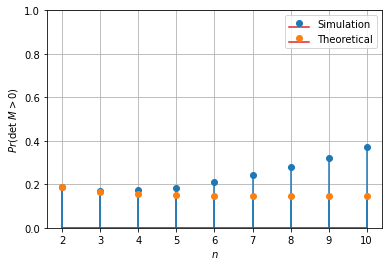
\includegraphics[width=8cm]{Fig2.png}
    \caption{Plot for Simulation v/s Theoretical}
    \label{fig:plot}
\end{figure}
\end{document}
